\documentclass[a4paper, 12pt]{article}

\usepackage{amsthm}
\usepackage{amsmath}
\usepackage{amssymb}
\usepackage{mathrsfs}
%\usepackage[latin1]{inputenc}
\usepackage[utf8]{inputenc}
\usepackage[T1]{fontenc}
%\usepackage{lmodern}
\usepackage{eurosym}
\usepackage[frenchb]{babel}
\usepackage{graphicx}
\usepackage{xcolor}

\title{Projet tutoré \\ \small\textit{Evaluation de mi-parcours}}
%\date{27/02/2014}

\begin{document}

\maketitle

\section{Préambule}
Notre sujet, de numéro inconnu, possède le titre provisoire suivant :
\begin{center}
	\emph{\og Reconnaissance du niveau de pollution d’une masse d’eau par images satellite grâce à un classificateur linéaire de type réseau de neurones formel \fg}
\end{center}
Il est traité par l'équipe suivante, du groupe ASPE :
\vspace{0.3cm}
\begin{itemize}
	\item Gabriel \textsc{Augendre}
	\item Philippe \textsc{Giraudeau}
	\item Sarah \textsc{Kugel}
	\item Adrien \textsc{Rabian}
	\item Quentin \textsc{Vaudaine}
\end{itemize}

\section{Contexte}
La région des Dombes dans l'Ain près de Bourg en Bresse possède une quantité importante de lacs et bassins tous interconnectés. Beaucoup de ces lacs et bassins se situent à proximité de champs agricoles. Ces champs étant utilisés de manière intensive, le recours à des pesticides et engrais chimique est souvent le meilleur moyen pour les agriculteurs de garder un rythme de production conséquent.

Les bassins sont utilisés également pour la pisciculture. Les pisciculteurs voient malheureusement  leurs populations de poissons décimées par les algues qui arrivent lors du remplissage du bassin et prolifèrent sous certaines conditions. Les écologues ont identifié la raison de la prolifération de ces algues dans les bassins comme étant un milieu biochimique modifié par les engrais et pesticides utilisés par les agriculteurs. Le taux de pollution des terres et des eaux de cette région devient nécessairement une préoccupation pour les écologues du LEHNA.

Pour surveiller le taux de pollution des lacs, il est nécessaire de recourir à des prélèvements. Malheureusement, ceux-ci sont coûteux et chronophages.

\section{Notre rôle}
L’objectif est, grâce à un classificateur de type réseau de neurones, d’évaluer le plus finement possible le taux de pollution des bassins, en se basant sur les relevés effectués in situ sur un nombre limité de lacs et en les corrélant à des images satellite de la zone pour obtenir un indice de pollution pour chaque masse d’eau. Dans un second temps, le logiciel devra généraliser les résultats et obtenir pour chaque lac de la région des Dombes un indice de pollution. Ainsi, les utilisateurs de cet outil pourront obtenir à partir d'autres images plus récentes une estimation du taux de pollution pour chaque lac.

\section{Méthodologie}
Dans cette section, nous allons décrire la méthode de travail que nous employons afin de mener à bien notre projet.

Tout d'abord, des réunions d'équipe en session plénière permettent de déterminer les orientations du projet et les tâches à effectuer, ainsi que leur hiérarchisation et leur affectation. La supervision globale du projet s'effectue à l'aide de Redmine, application libre de gestion de projets, qui permet de saisir les tâches à effectuer et donc de centraliser l'avancée de celui-ci.

Ensuite, le travail s'effectue soit individuellement, soit en petits groupes de travail, quand le contexte est favorable, i.e. que du temps nous soit laissé à côté du planning de la formation, fort chargé au demeurant.
Une part importante de notre travail implique le recours à des technologies qui nous sont mal connues. A ce titre, nous devons donc d'abord nous familiariser avec celles-ci en procédant à des essais.

Par la suite, le développement proprement dit du code destiné à être inclus dans le livrable final est réalisé selon la méthode dite du \emph{\og Test Driven Development \fg}, qui consiste à écrire les tests pertinents relativement à la fonction remplie par une portion de code avant même l'écriture de celle-ci, et de vérifier que la production remplit effectivment lesdits tests.

Le code en question est versionné \textit{via} un dépôt Git, centralisé sur un serveur Gitlab afin de permettre un accès aisé par chacun des contributeurs.
Le système d'intégration continue TeamCity se charge ensuite de faire passer les tests sus-cités au code ainsi partagé afin de s'assurer que celui-ci :
\begin{enumerate}
	\item est valide eût égard aux objectifs fixés
	\item n'introduit pas de régression par rapport aux fonctionnalités précédentes.
\end{enumerate}
Toutes ces données sont centralisées sur un espace de discussion (Slack), et font l'objet de récapitulatifs réguliers par courriel.

\section{Outils \& technologies}
Le langage de programmation Python a été retenu pour l'écriture de ce projet. L'interpréteur de base sera secondé par les librairies suivantes, afin de pouvoir écrire toutes les fonctionnalités de notre programme :
\begin{description}
	\item[NumPy] Sert à la manipulation d’environnements numériques et tabulaires complexes, notamment les collections de pixels des images SPOT
	\item[PyBrain] Pour effectuer des tests sur des réseaux de neurones existants, afin d'en préparer notre propre implémentation
	\item[OpenCV] Nous permet de manipuler les images SPOT
	\item[GDAL] La \emph{Geospatial Data Abstraction Library} permet de gérer les données géographiques associées aux images SPOT. On utilisera également les bindings pour le langage Python, afin d'effectuer les liaisons \textit{inter se} des fonctions des modules Python et des fonctions natives complilées en C.
\end{description}

En outre, le framework PyTest est utilisé pour l'éxécution des tests unitaires, et le processus de build et de gestion des dépendances est pris en charge par PyBuilder.

Tous ces outils étant totalement en dehors du cadre de la formation dispensée à l'IUT, nous avons dû consacrer un temps considérable à se documenter et à expérimenter sur iceux. Pour ce faire, nous avons essentiellement utilisé les documentations développeur et utilisateur, ainsi que d'autres ressources en ligne quand nous pouvions en trouver. A titre d'exemple, pour l'apprentissage du langage Python, nous avons pu nous référer aux cours proposés par des MOOCs, comme OpenClassroom (\textit{ex} Site du Zéro).

\section{Etat du travail}
\subsection{Avancement actuel}
Ainsi que nous l'avons précédemment mentionné, nous avons dû faire face à un travail de recherche préliminaire que nous avions considérablement sous-estimé. En conséquence, le travail de codage du cœur applicatif est retardé d'autant. Actuellement, nous estimons entre six et dix semaines le retard induit par les recherches sur l'état de l'art et par le datamining des images SPOT.

Ainsi, nous sommes aujourd'hui en état d'affirmer que cette phase est en passe d'être close (cf. diagramme \ref{gantt}, page \pageref{gantt}), et de vous livrer nos rôles jusqu'ici.

Sarah \textsc{Kugel} et Philippe \textsc{Giraudeau} étant issus d'un cursus académique lié aux sciences cognitives, ils se sont chargés des recherches sur la partie intelligence artificielle du projet, ainsi que de l'instruction de leurs collaborateurs en la matière et de la modélisation du problème et des solutions que nous y apporterons.

Quentin \textsc{Vaudaine} a pris en charge l'étude des données qui nous ont été fournies, ainsi que les recherches sur les librairies à même de les traiter.

Adrien \textsc{Rabian} et Gabriel \textsc{Augendre} ont quand à eux commencé le codage du projet, déterminé la méthodologie, mis en place les outils de travail collaboratif et les ont adaptés aux contraintes du projet. Ils ont, en outre, formé leurs collaborateurs à leur usage.

\subsection{Planification future}
Nous devons désormais réaliser le cœur du programme, à savoir son intelligence artificielle. Nous nous attendons à devoir tâtonner avant d'obtenir une IA fonctionnelle. En parallèle de cela, nous devons également programmer les \og à côté \fg ~ du noyau, à savoir l'IHM, la préparation des données fournies pour qu'elles soient exploitables par l'IA, etc.

En outre, nous devons faire face au départ de Sarah \textsc{Kugel} depuis le 18/03/2015. En sa qualité de diplômée en sciences cognitives, elle constituait l'un des socles sur lesquels s'appuie le cœur de notre projet, ce qui nous rend son départ fort préjudiciable pour l'avancée du projet.

\section{Achèvement marquant}
\textsl{Devra être déterminé par l'équipe avant rédaction.}

\newpage
\appendix
\section{Ressources}
	\begin{figure}
		\begin{center}
			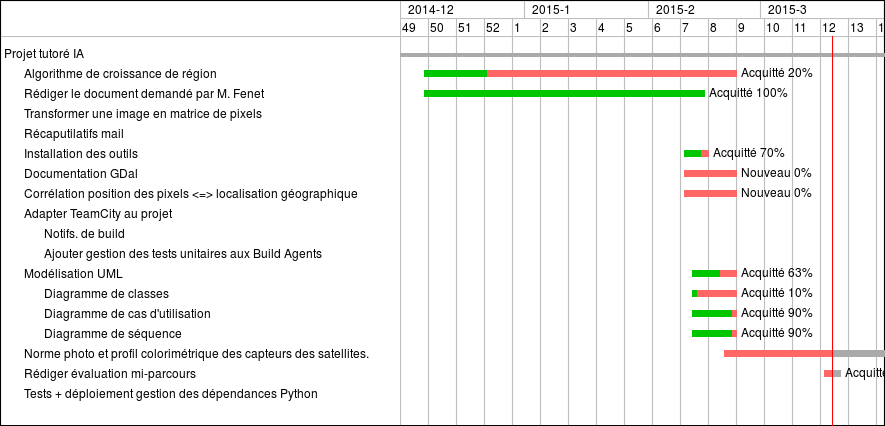
\includegraphics[height=60mm]{gantt.png}
			\newline
			\caption{Diagramme de Gantt au 18/03/2015}
			\label{gantt}
		\end{center}
	\end{figure}

\end{document}
